\documentclass{article}
\usepackage[a4paper,top=0.75in, bottom=0.75in, left=1in, right=1in,footskip=0.2in]{geometry}
%\usepackage{fullpage}
%-----------------Hyperlink Packages--------------------
\usepackage{hyperref}
\hypersetup{
	 colorlinks   = true,
     citecolor    = black,
     linkcolor    = black,
     urlcolor     = black
}
%-----------------Figure Packages--------------------
\usepackage{graphicx}                       % For figures
%\usepackage{epsfig} % for postscript graphics files
%------------------Math Packages------------------------
\usepackage{amssymb,amsmath}
\usepackage{textcomp}
\usepackage{mdwmath}
\usepackage{mdwtab}
\usepackage{eqparbox}
%------------------Table Packages-----------------------
\usepackage{rotating}                     % Used to rotate tables
\usepackage{array}                        % Fixed column widths for tables
%-----------------Algorithm Packages--------------------
\usepackage{listings}                     % Source code
\usepackage{algorithm}                    % Pseudo Code
\usepackage{algpseudocode}
%---------------------------------------------------------
\setcounter{tocdepth}{3}
%opening

\begin{document}

\title{
Artificial Intelligence Project 2 \\
Decision Tree
}
\author{Class 1, Team 6}
\date{\today}
\maketitle
\tableofcontents

\section{Team Members}

\begin{table}[H]
\centering
\begin{tabular}{l l l}
Name & Student ID  & Job\\
\hline
Fan Ziyao & 12330081 & Team leader, implementation\\
Chen Yingcong & 12330049 & Implementation \\
Chen Xiongtao & 12330040 & Modeling, implementation \\
Huang Long & 12330132 & Implementation \\
Zhang Qiuyi & 12330402 & Implementation, documentation

\end{tabular}
\end{table}

\section{Problem Description}

The dataset (including the training set and the test set) contains clean data generated from $8 \times 8$ images of handwritten digits. Each record contains the sampled data of size $8 \times 8 = 64$ (each point ranging in $[0, 16]$) and its label (range $[0, 9]$).

Given this dataset, the goal is to build a neural network with the training set and evaluate its precision by classifying the records in the test set (that is, to predict its label based on its sampled data).

\section{Algorithm and Implementation}

For this project we implemented a multilayer perceptron(MLP) with the logistic function

$$y(v_i) = (1+e^{-v_i})^{-1}$$

as the activation function.

\subsection{Building the Neural Network}

First we initialize the neural network with random weights ranging between $[-0.25, 0.25]$ (it is just a empirical value). Then, we use back propagation for training the network. Here instead of running the backpropagation on the training data sequantially, we randomly choose records from the training data to propagate. The algorithm is discribed in Algorithm~\ref{alg:train}.

The back propagation, as shown in Algorithm~\ref{alg:bp}, will be run until a certain number of epochs is reached.

\begin{algorithm}[H]
\centering
\caption{Training the Network}
\label{alg:train}
  \begin{algorithmic}[1]
    \Function{Training}{$examples$, $epochs$}
    	\State Initiailize $network$ with random weights between $[-0.25, 0.25]$
    	\For{$k = 1 \to epochs$}
   	    	\State Randomly choose a record $(\mathbf{x}$, $\mathbf{y})$ from $examples$
   	    	\State \Call{Back-Propagate}{$\mathbf{x}$, $\mathbf{y}$, $network$}
    	\EndFor
    \EndFunction
  \end{algorithmic}
\end{algorithm}

\begin{algorithm}[H]
\centering
\caption{Back Propagation}
\label{alg:bp}
  \begin{algorithmic}[1]
    \Function{Back-Propagate}{$\mathbf{x}$, $\mathbf{y}$, $network$}
    	\Comment $\mathbf{x}$ is the input
    	\State $w \gets network.weights$ \Comment $\mathbf{y}$ is the vector transformed from the label
    	\For{each node $i$ in the input layer} 
    		\State $a_i \gets x_i$
    	\EndFor
    	
    	\For{$l = 2 \to L$}  \Comment $L$ is the number of layers in the network
    		\For{each node $j$ in layer $l$}
    			\State $in_j \gets \sum_i w_{i,j}a_i$
    			\State $a_j \gets g(in_j)$  \Comment $g$ is the activation fucntion
    		\EndFor
    	\EndFor

		\For{each node $j$ in the otput layer}
			\State $\Delta[j] \gets g'(in_j) \times (y_j - a_j)$
			\Comment $\Delta$ is a local vector of erros indexed by network node
		\EndFor
		
		\For{$l = L - 1 \to 1$}
			\For{each node $i$ in layer $l$}
				\State $\Delta[i] \gets g'(in_i) \sum_j w_{i,j}\Delta[j]$
				\Comment propagate backwords
			\EndFor
		\EndFor
		
		\For{each weight $w_{i,j}$}
			\State $w_{i,j} \gets w_{i,j} + \alpha \times a_i \times \Delta[j]$  \Comment gradient descent rule, $\alpha$ is the learning rate
		\EndFor
		
		\State $network.weights \gets w$
    \EndFunction
  \end{algorithmic}
\end{algorithm}

\subsection{Classification}

The algorithm for classifying an observation is described in Algorithm~\ref{alg:cla}. Note that the output is a vector, its value needs to be further interpreted.

\begin{algorithm}[H]
\centering
\caption{Classification}
\label{alg:cla}
  \begin{algorithmic}[1]
    \Function{Classify}{$network$, $observation$}
    	\State $w \gets network.weights$
    	\State $a \gets observation$
    	\For{$l = 2 \to L$}  \Comment $L$ is the number of layers in the network
    		\For{each node $j$ in layer $l$}
    			\State $in_j \gets \sum_i w_{i,j}a_i$
    			\State $a_j \gets g(in_j)$  \Comment $g$ is the activation fucntion
    		\EndFor
    	\EndFor
    	\State \Return $a$
    \EndFunction
  \end{algorithmic}
\end{algorithm}

\section{Experiment Result}

For this project, we set the number of layers in the neural network to $3$ (i.e. one input layer, one hidden layer, one output layer), and the learning rate $\alpha$ is set to $0.2$. Before building the neural network, we first transform the labels into vectors. Every elements in the vector is first set to 0, then the element with the same index as the lable will be set to 1. For example, when the label is $0$, we transform it into a vector:

$$[1, 0, 0, 0, 0, 0, 0, 0, 0, 0]$$

Then, the input layer consists of vectors of size $64$, and the output layer consists of vectors of size $10$. The output vectors contains the probabilities for each label, here we choose the label with the largest probability as the final result.

\paragraph{We evaluate the implementation from two different perspectives.} First, we examine the relationship between its precision and the size of the training data (i.e. the learning curve), as shown in Figure ~\ref{fig:curve}. The number of hidden units is set to $50$, and we stop the iteration after $50,000$ epochs. When the size of training data is larger than $1000$, the precision stays higher than $90\%$. Generally the precision increases with the size of training data, but there are signs of overfitting.

Then, we examine the relationship between the total errors produced by the neural network and the number of epochs. Here we use the full training data set and set the number of hidden units to $50$. As shown in Figure ~\ref{fig:error}, The number of errors decreases significantly when the epochs grows large enough. When the number of epochs becomes larger than $20, 000$, the number of errors stays at about $100$ (given that the size of the test set is about $1,700$, this implies that the precision stays over $90\%$).

\begin{figure}[H]
\centering
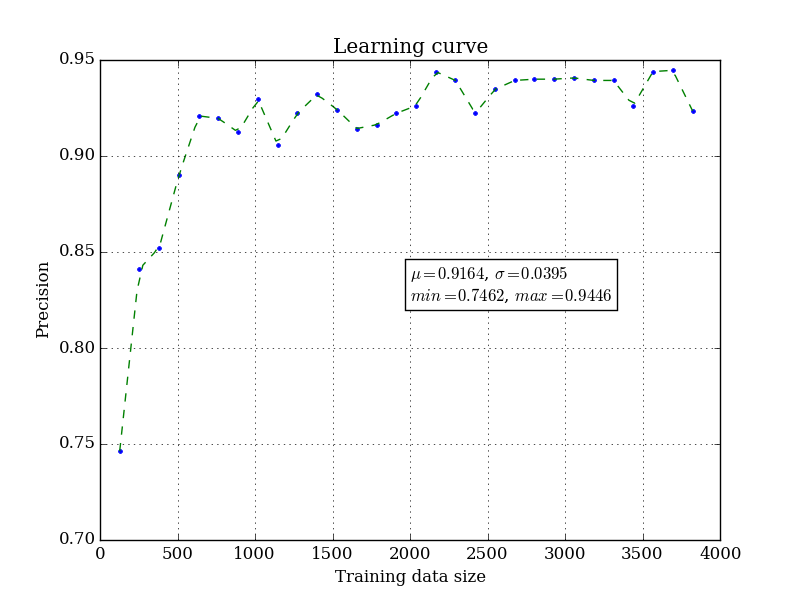
\includegraphics[width=400pt]{../asset/learning-curve.png}
\caption{Learning Curve}
\label{fig:curve}
\end{figure}

\begin{figure}[H]
\centering
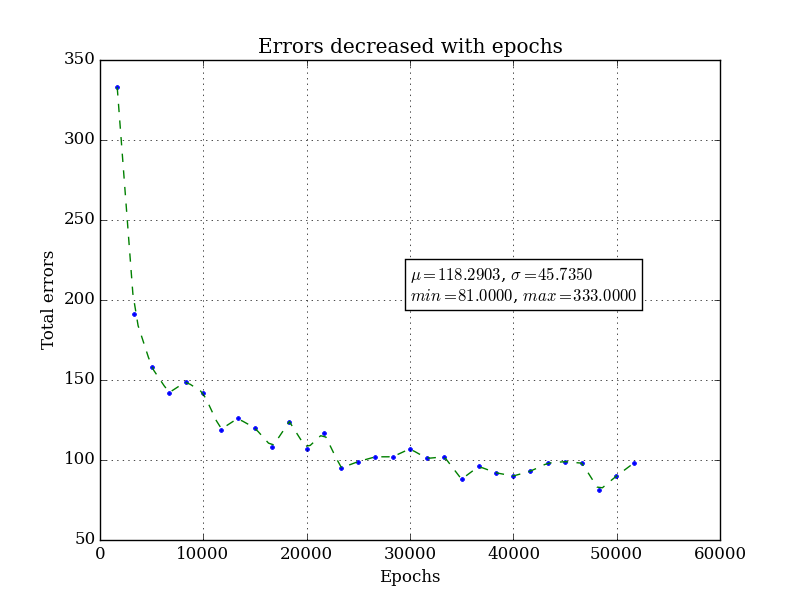
\includegraphics[width=400pt]{../asset/error-curve.png}
\caption{Relationship between total errors and epochs}
\label{fig:error}
\end{figure}

\end{document}
